
\documentclass[]{article}
\usepackage[a0paper]{geometry}
\pagenumbering{gobble}
\usepackage{tikz}
\usepackage{amsmath}
\usetikzlibrary{shapes, arrows, positioning}
\begin{document}
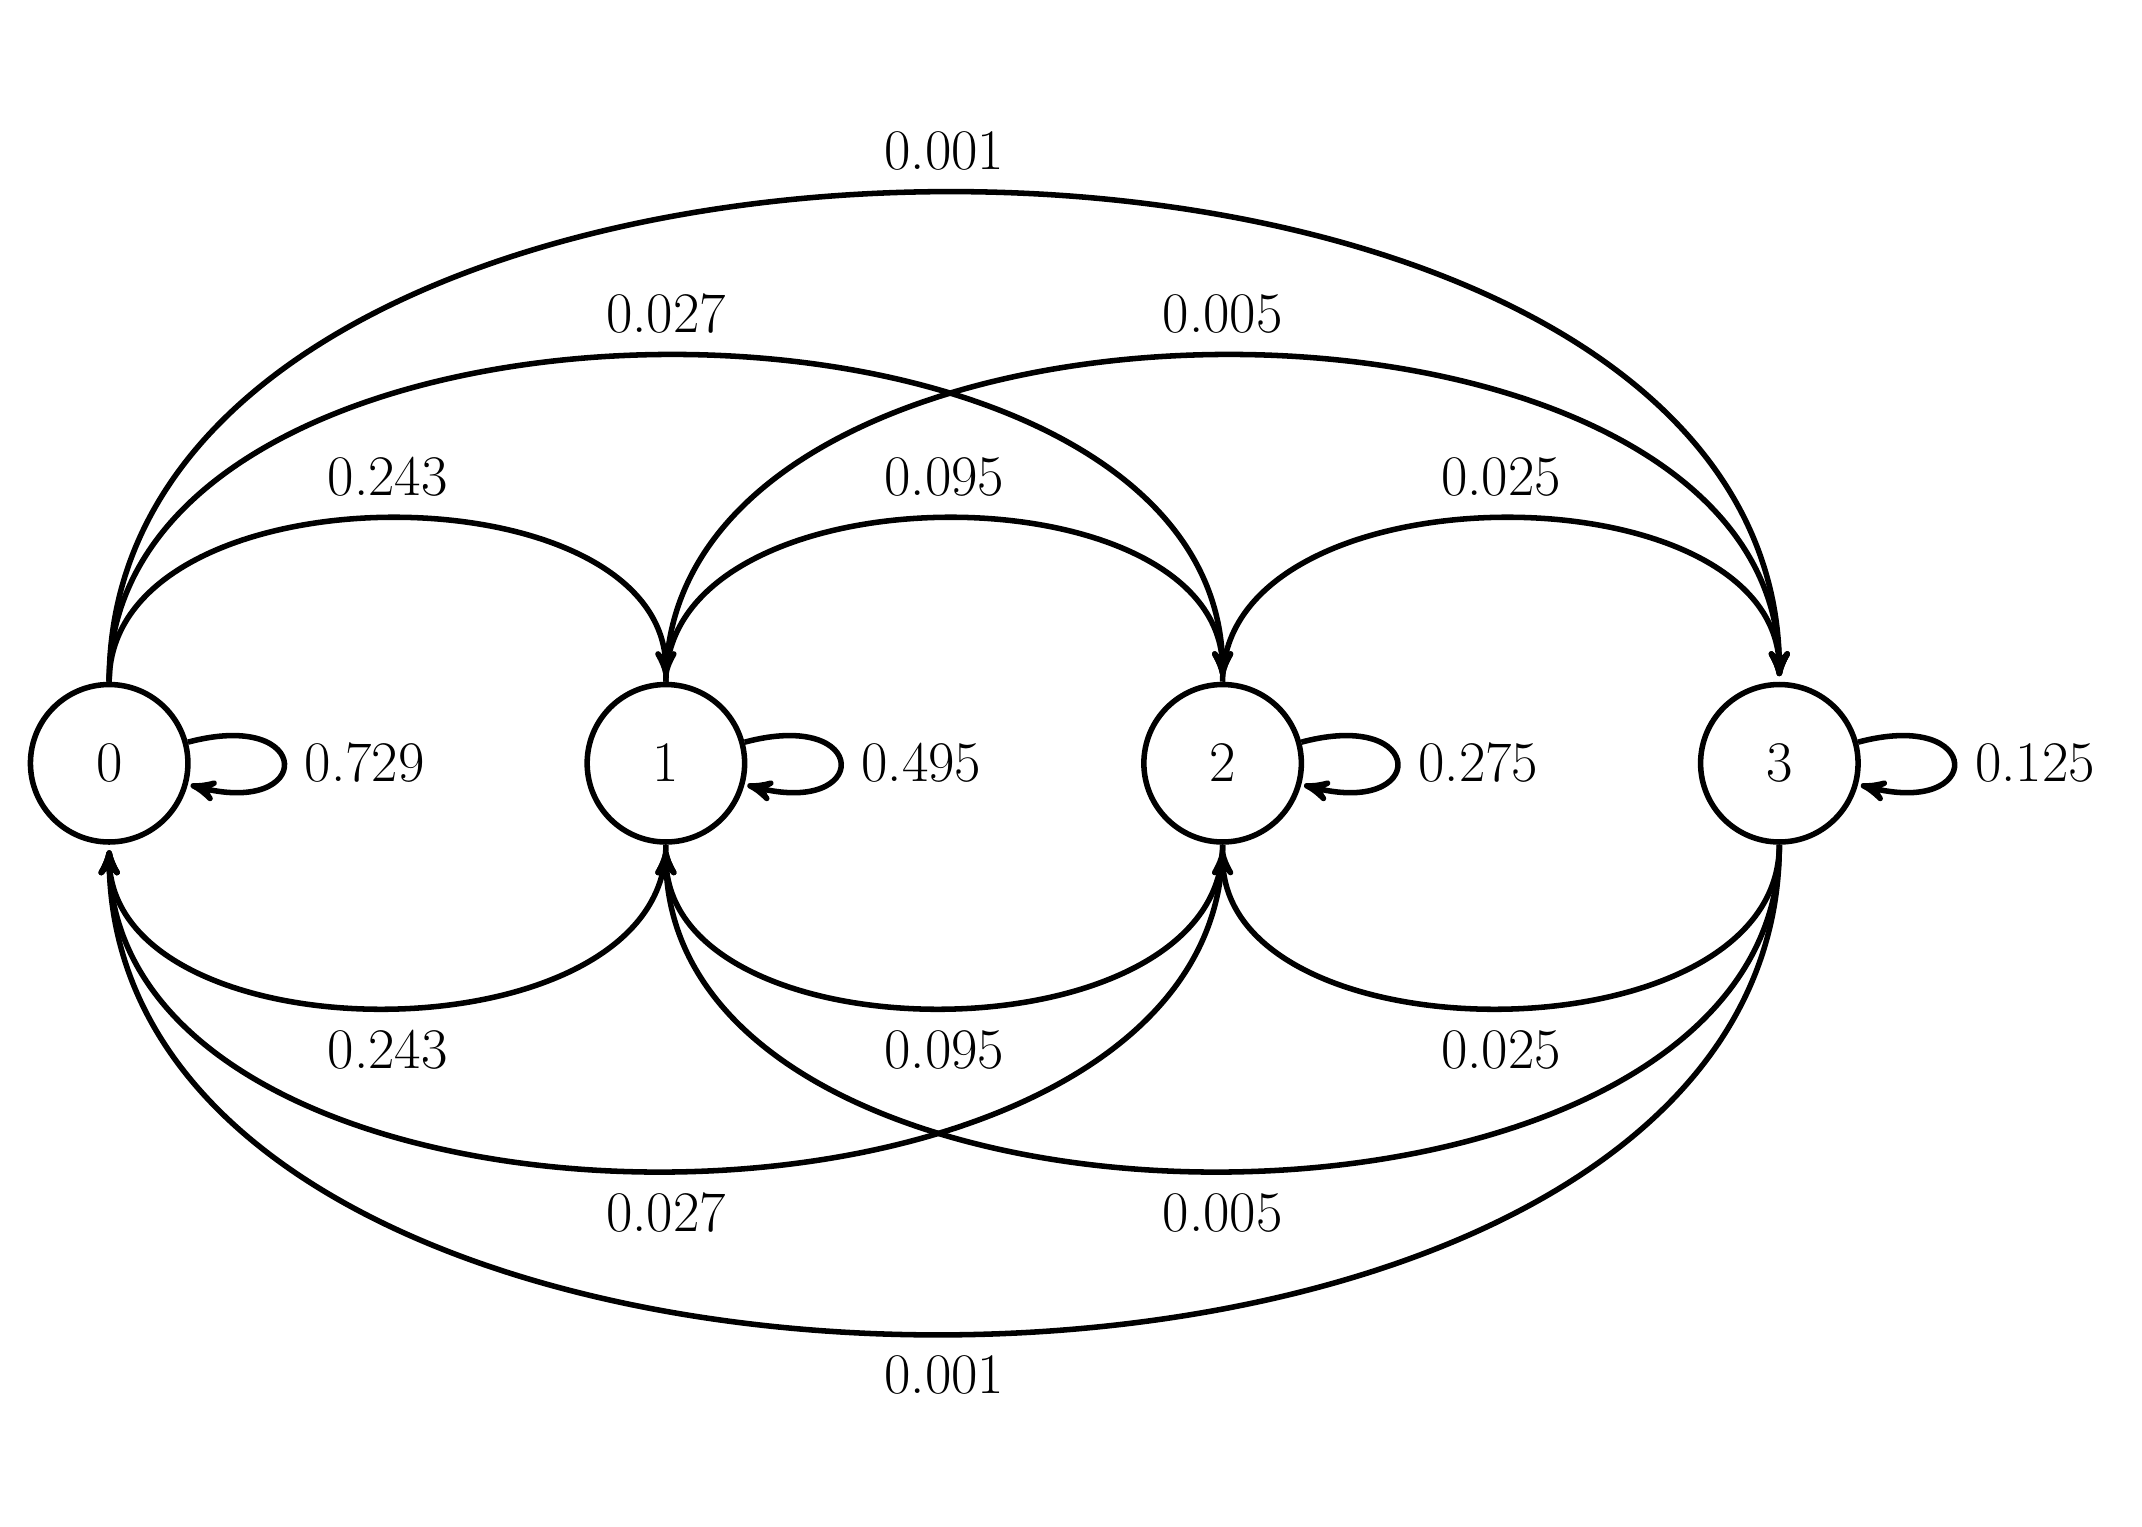
\begin{tikzpicture}[->,>=stealth',shorten >=2pt, line width=2pt, node distance=5cm, style = {minimum size = 20mm}]
\tikzstyle{every node}=[font =\huge]
\node[circle, draw](n0){0};
\node[circle, draw](n1)[right = of n0] {1};
\node[circle, draw](n2)[right = of n1] {2};
\node[circle, draw](n3)[right = of n2] {3};
\path(n0) edge [loop right] node {0.729} (n0);
\draw[->] (n0) to [out=90, in=90, edge node={node [above=-.5cm] {0.243}}] (n1);
\draw[->] (n0) to [out=90, in=90, edge node={node [above=-.5cm] {0.027}}] (n2);
\draw[->] (n0) to [out=90, in=90, edge node={node [above=-.5cm] {0.001}}] (n3);
\draw[->] (n1) to [out=-90, in=-90, edge node={node [below=-.5cm] {0.243}}] (n0);
\path(n1) edge [loop right] node {0.495} (n1);
\draw[->] (n1) to [out=90, in=90, edge node={node [above=-.5cm] {0.095}}] (n2);
\draw[->] (n1) to [out=90, in=90, edge node={node [above=-.5cm] {0.005}}] (n3);
\draw[->] (n2) to [out=-90, in=-90, edge node={node [below=-.5cm] {0.027}}] (n0);
\draw[->] (n2) to [out=-90, in=-90, edge node={node [below=-.5cm] {0.095}}] (n1);
\path(n2) edge [loop right] node {0.275} (n2);
\draw[->] (n2) to [out=90, in=90, edge node={node [above=-.5cm] {0.025}}] (n3);
\draw[->] (n3) to [out=-90, in=-90, edge node={node [below=-.5cm] {0.001}}] (n0);
\draw[->] (n3) to [out=-90, in=-90, edge node={node [below=-.5cm] {0.005}}] (n1);
\draw[->] (n3) to [out=-90, in=-90, edge node={node [below=-.5cm] {0.025}}] (n2);
\path(n3) edge [loop right] node {0.125} (n3);

\end{tikzpicture}
\end{document}
